\documentclass[border=6pt]{standalone}
\usepackage{tikz}
\usetikzlibrary{arrows.meta}
\begin{document}
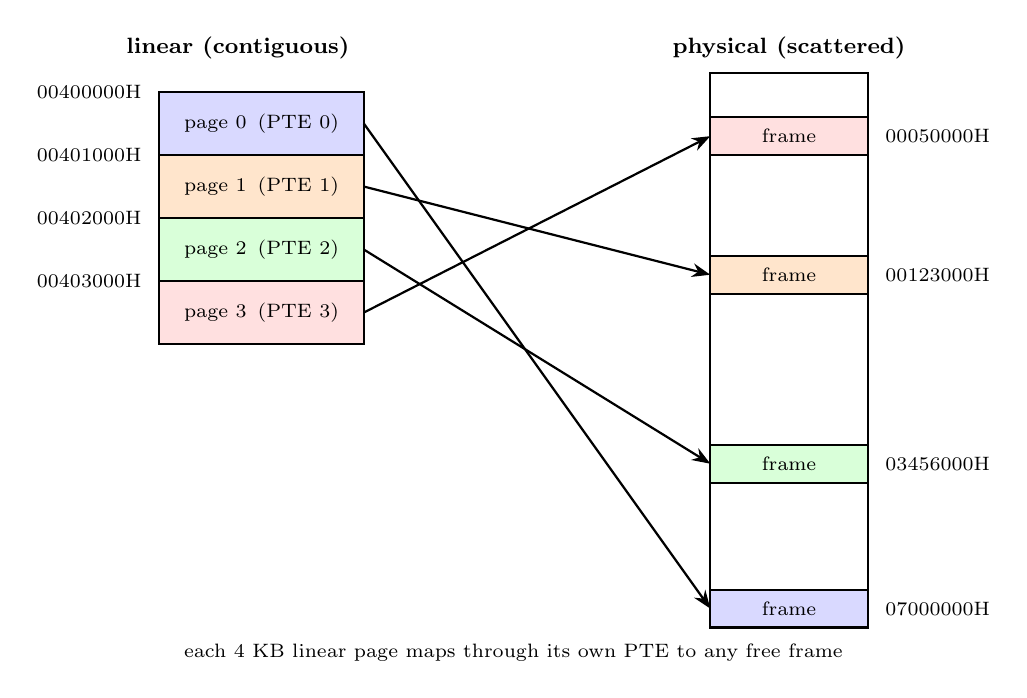
\begin{tikzpicture}[>=Stealth,font=\small,y=0.8cm]
\node[font=\footnotesize\bfseries] at (1.0,4.7) {linear (contiguous)};
\foreach \i/\a/\c in {0/00400000H/blue!15,1/00401000H/orange!20,2/00402000H/green!15,3/00403000H/red!12} {
  \draw[thick,fill=\c] (0,3-\i) rectangle (2.6,4-\i);
  \node[font=\scriptsize] at (1.3,3.5-\i) {page \i\enspace(PTE \i)};
  \node[font=\scriptsize,anchor=east] at (-0.1,4-\i) {\a};
}
\node[font=\footnotesize\bfseries] at (8.0,4.7) {physical (scattered)};
\draw[thick] (7,4.3) rectangle (9,-4.5);
\foreach \y/\a/\c/\i in {3.6/00050000H/red!12/3,1.4/00123000H/orange!20/1,-1.6/03456000H/green!15/2,-3.9/07000000H/blue!15/0} {
  \draw[thick,fill=\c] (7,\y) rectangle (9,\y-0.6);
  \node[font=\scriptsize] at (8,\y-0.3) {frame};
  \node[font=\scriptsize,anchor=west] at (9.1,\y-0.3) {\a};
}
\draw[->,thick] (2.6,3.5) -- (7,-4.2);
\draw[->,thick] (2.6,2.5) -- (7,1.1);
\draw[->,thick] (2.6,1.5) -- (7,-1.9);
\draw[->,thick] (2.6,0.5) -- (7,3.3);
\node[font=\scriptsize,anchor=north] at (4.5,-4.6) {each 4 KB linear page maps through its own PTE to any free frame};
\end{tikzpicture}
\end{document}
